\documentclass[journal]{IEEEtran}
\IEEEoverridecommandlockouts
% The preceding line is only needed to identify funding in the first footnote. If that is unneeded, please comment it out.
\usepackage{cite}
\usepackage{bm}
\usepackage{amsmath,amssymb,amsfonts}
\usepackage{algorithm} 
\usepackage{titlesec}
\usepackage{algpseudocode}
\usepackage{graphicx}
\usepackage{mdframed}
\usepackage{enumerate}
\usepackage{textcomp}
\usepackage{xcolor}
\usepackage{svg}
\usepackage{tabularx,booktabs}
\usepackage{caption}
\usepackage{xcolor}
\usepackage{subcaption}

\newcolumntype{C}{>{\centering\arraybackslash}X} 
\setlength{\extrarowheight}{1pt} % for a bit more open "look"
\usepackage{lipsum} % filler text

\newcommand{\name}{TraDWin}

% Redefine the format for subsection numbering
% \renewcommand{\thesubsection}{\arabic{subsection}.}

% Redefine the format for subsubsection numbering
% \renewcommand{\thesubsubsection}{(\roman{subsubsection})}

% Adjust the formatting of subsection titles to be bold
% \usepackage{titlesec}
% \titleformat{\subsection}{\bfseries}{\thesubsection}{1em}{}

% Adjust the formatting of subsubsection titles to be bold
% \titleformat{\subsubsection}{\bfseries}{\thesubsubsection}{1em}{}

\def\BibTeX{{\rm B\kern-.05em{\sc i\kern-.025em b}\kern-.08em
    T\kern-.1667em\lower.7ex\hbox{E}\kern-.125emX}}
\begin{document}



\title{\name: An interactive Digital Twin for City Traffic}

% \author{
%     \IEEEauthorblockN{Shreyansh Yadav}
%     \IEEEauthorblockA{\textit{Department of Computer Science Engineering} \\
%     \textit{IIT BHU, Varanasi}\\
%     India \\
%     shreyansh.yadav.cse19@itbhu.ac.in}
%     \and
%     \IEEEauthorblockN{Dr. Vignesh Sivaraman}
%     \IEEEauthorblockA{\textit{Assistant Professor} \\
%     \textit{Department of Computer Science and Engineering} \\
%     \textit{IIT BHU, Varanasi}\\
%     India \\
%     vignesh.cse@iitbhu.ac.in}
% }
\author{
Shreyansh Yadav, Vignesh Sivaraman, \textit{Member, IEEE} and Vignesh Sridharan, \textit{Member, IEEE}
\IEEEcompsocitemizethanks{S. Yadav and V. Sivaraman are associated with 
the Department of Computer Science and Engineering, Indian Institute of Technology, (BHU) Varanasi, India.\\
V. Sridharan is associated with Institute for Infocomm Research (I$^2$R), A*STAR, Singapore.\\
(E-mail: shreyansh.yadav.cse19@itbhu.ac.in, vignesh.sivaraman@u.nus.edu and shreyansh.yadav.cse19@itbhu.ac.in)
}
}
\maketitle

% Vignesh: I have broken the paper into smaller files for easier edit. You can open the corresponding file and make changes.

\begin{abstract}

ChatGPT
In the contemporary world characterized by rapid urbanization and burgeoning populations, cities worldwide confront pressing challenges, notably the effective management of traffic congestion and the optimization of transportation infrastructure. The advent of smart cities facilitated by 5G and the Internet of Things (IoT) has unlocked unprecedented opportunities to harness real-time data. This technological advancement has spurred the adoption of sophisticated cyberphysical systems such as Digital Twins, which are increasingly recognized for their potential in modeling urban traffic dynamics with precision.

This study introduces \name, a Traffic Digital Twin (TDT) designed to seamlessly aggregate real-time traffic data sourced from diverse sensors, cameras, GPS devices, and analogous instruments. By leveraging physics-informed deep machine learning models, our framework represents a departure from traditional empirical approaches reliant on laborious and resource-intensive micro-simulations. The TDT integrates comprehensive datasets encompassing road network configurations, traffic volumes at distinct junctures, and contextual parameters including road characteristics and meteorological conditions. It is specifically engineered and validated to address three pivotal aspects of urban traffic state estimation: (i) prediction of future traffic conditions, (ii) imputation of traffic state data for segments with missing information, and (iii) traffic assignments in response to evolving map topologies, crucial for scenarios such as road closures or urban development initiatives. Finally, we evaluate our proposed model using traffic volume data obtained from Dublin city's SCATS traffic management system, alongside simulation-based assessments using the SUMO platform to replicate pertinent scenarios.
\end{abstract}
%!Tex root=./paper.tex
\section{Introduction}

The contemporary landscape of urban development is characterized by rapid urbanization and increasing population densities, presenting formidable challenges in optimizing traffic flow and urban infrastructure planning. Extensive research has documented the multifaceted impacts of traffic on public health\cite{levy2010evaluation}, economic viability\cite{gorea2016financial}, and social dynamics\cite{anciaes2017social}, highlighting the urgent need for advanced technological interventions.


The Digital Twin, as an emerging concept within cyber-physical systems (CPS), has garnered significant attention over the past decade, particularly with the advancements in big data, IoT connectivity, and affordable computing, which have rendered such systems increasingly practical\cite{guo2017mobile}\cite{singh2021digital}. A Digital Twin is a virtual representation of a real-world object, system, or process, meticulously designed to replicate its physical counterpart in the digital realm\cite{VANDERHORN2021113524}. This enables the Digital Twin to capture and simulate the intricate details of a physical entity, facilitating real-time monitoring, analysis, and prediction of its behavior. It transcends traditional 3D modeling by incorporating live data, sensor inputs, and advanced analytics, thereby providing a dynamic and interactive digital mirror of the physical world\cite{VANDERHORN2021113524}. This capability has found applications across a multitude of fields, including manufacturing, engineering, healthcare, urban planning, and beyond.

Our traffic digital twin, \name, serves as an interactive simulation of city traffic, continuously updating its internal state with real-time data from various sources. The proliferation of smart cities, equipped with IoT sensors and live camera feeds, has led to the development of numerous methodologies to enhance this capability. For example, the Sydney Coordinated Adaptive Traffic System (SCATS)\cite{scats} employs inductive loop-based sensors at traffic signals to monitor traffic volumes and is operational in over 180 cities across 28 countries, including New Zealand, Dublin, Shanghai, and Hong Kong\cite{wiki:sydney_traffic_system}. Cities such as New York and Los Angeles have implemented systems similar to SCATS. Additional techniques involve traffic probes\cite{zhu2012probe}, GPS-enabled mobile phones\cite{rose2006mobile}, exemplified by Google’s provision of congestion and travel time data, and deep learning computer vision models that utilize cameras to identify and count vehicles. These methods, however, primarily provide absolute volume counts at various nodes, rather than more granular data such as source-destination pairs, which present logistical and privacy challenges. In our study, we rely exclusively on absolute traffic volume data, without incorporating any information related to individual vehicles.

In the contemporary literature review, as discussed subsequently, mathematical and deep learning time series analysis methods prevail for tasks (i) and (ii). However, for task (iii), microscopic traffic simulation software such as SUMO \cite{sumo} and Vissim \cite{vissim} are commonly utilized. These simulation engines are computationally intensive and require detailed information on vehicle types, origins, and destinations to produce accurate results, which may pose challenges in data acquisition. Another notable limitation of previous approaches, which predominantly focus on time series analysis, is their exclusive consideration of traffic flow data without accounting for potential exogenous variables such as weather \cite{weather}, holidays \cite{holiday}, and other contextual factors.

We argue that traffic dynamics are shaped by both intrinsic data relationships and external factors such as weather \cite{weather} and holidays \cite{holiday}. Moreover, there may be latent relationships among these variables that are not immediately evident. Thus, our proposed TDT framework is designed to be highly adaptable, allowing for the inclusion of new features to enhance its predictive capacity.

In this paper, we aim to provide an end-to-end framework that first collects and aggregates real-time traffic data. Our proposed framework utilizes the aggregated data to address three key tasks related to traffic modeling:
\begin{enumerate}[(i)]
\item \textbf{Traffic Prediction}: Predicting how traffic volume will change in the future based on a given traffic volume time series and historical data.
\item \textbf{Imputation}: For traffic volume time series with missing data (potentially due to sensor failure or other issues), our framework aims to accurately fill in the missing values.
\item \textbf{Re-assignment on Edge Addition or Removal}: Our objective is to predict how traffic flow will be affected by changes in the road network, such as the addition or removal of road segments.
\end{enumerate}

Our proposed framework (i) takes input a graph representation of map where different regions are the vertices of the graph and different roads form the edges of the graph. (ii) Next, it encodes the structural features of graph nodes using Node2Vec \cite{node2vec} and  transforms them into feature embeddings. (iii) These embeddings are augmented with relevant traffic data and other semantic information, such as weather, encoded using Word2Vec \cite{word2vec}.
(iv) This encoded representation of the graph is used as input to an informed Wasserstein distance-based Generative Adversarial Imputation Net (GAIN), a modified version of the GAIN \cite{gain}, which is a type of conditional GAN. This adaptation incorporates elements from the Wasserstein GAN (WGAN) \cite{wgan}, enhancing GAN training effectiveness. Additionally, we integrate a modified loss function from physics-informed deep learning techniques \cite{pidl}, ensuring the model adheres to physical conservation laws.
(v) This proposed model is trained using real-world data and the trained model is used compute the tasks of prediction, imputation, and re-assignment of traffic.

To summarize, we outline the our contributions as follows:

\begin{enumerate}[(i)]
\item We introduce an end-to-end workflow for an interactive Traffic Digital Twin system that utilizes traffic volume data as its primary input.
\item Our proposed framework considers contextual data like geographical, meteorological, temporal data that are aggregated according to physcial conservation laws.
\item We mathematically capture the dynamics involved in traffic modeling using physical laws.
\item Using this physics-informed traffic model, we develop a Wasserstein distance-based Generative Adversarial Imputation Net (GAIN) framework to predict and compute various tasks using real-world traffic data.
\end{enumerate}

The rest of the paper is organized as follows. The literature review is presented in Section~\ref{sec:related-works}. We formulate our problem in Section~\ref{sec:problem-for}. Our proposed framework is presented in Section~\ref{sec:system-model}. We present our empirical findings and performance evaluation of our proposed framework in Section~\ref{sec:experiments}. Finally, Section~\ref{sec:conclusion} concludes the paper.

%!TEX root=./paper.tex
\section{Related Work}\label{sec:related-works}

In this section, we review the existing literature on traffic modeling, focusing on current spatio-temporal modeling methods. We compare these approaches with our framework, addressing recent work relevant to each of the specific tasks our model aims to perform: prediction, imputation, and prediction in response to changing topology, the latter being a distinctive feature of our work.

Autoregressive Integrated Moving Average (ARIMA) \cite{arima} and its variants, such as time-oriented ARIMA \cite{time_arima} and Seasonal ARIMA \cite{sarima}, are widely used traditional algorithms for prediction and forecasting tasks. ARIMA operates on time series data and is frequently combined with other algorithms to incorporate spatial features. For instance, C. Xu et al. \cite{Xu2016} integrated ARIMA with a genetic algorithm to estimate future traffic flow on roads. While ARIMA models are proficient in capturing linear time series data, the addition of genetic algorithms enhances their ability to extract features from nonlinear historical data. This integration demonstrates the versatility and adaptability of ARIMA-based approaches in addressing complex prediction challenges. Consequently, we also compare our model's performance with that of the ARIMA model. But one major problem this method suffers from is the lack of spatial information about the road network, which is crucial for traffic prediction tasks.

Other methods, such as Temporal Regularized Matrix Factorization (TRMF) \cite{trmf}, Bayesian Temporal Regularized Matrix Factorization (BTRMF) \cite{btrmf}, and Bayesian Temporal Matrix Factorization (BTMF) \cite{btrmf}, have also been explored in the context of traffic prediction. These methods extend the principles of matrix and tensor factorization to capture temporal dependencies and spatial correlations in high-dimensional traffic data.

TRMF, introduced by Lai et al. (2017), extends matrix factorization to tensor data structures, enabling the modeling of multi-dimensional traffic flow data with enhanced flexibility. Similarly, BTRMF, proposed by Liu et al. (2019), integrates Bayesian inference into tensor factorization to provide probabilistic predictions and uncertainty quantification in traffic forecasting tasks. BTMF and Bayesian Temporal Tensor Factorization (BTTF) further extend the Bayesian framework to matrix and tensor factorization, respectively, offering robust approaches for modeling temporal dynamics and spatial interactions in traffic networks while accounting for uncertainties in the prediction process.

These methods contribute to the diverse landscape of predictive models for traffic forecasting, each offering unique advantages and insights for accurately addressing the challenges of traffic flow prediction. But again, these methods are limited in their ability by the lack of spatial information about the road network, as was the case with ARIMA.
Next, we explore GNNs which is a new class of models that try to address this limitation.

Graph Neural Networks (GNNs) \cite{gnn} have emerged as a prominent tool for spatiotemporal modeling, demonstrating effectiveness in various applications such as traffic forecasting and imputation. Studies by Li et al. (2018) \cite{li2018gnn} and Zhang et al. (2019) \cite{wavenet} have highlighted their utility in accurately predicting traffic patterns and filling in missing data in traffic volume time series. GNNs iteratively update node representations based on local neighborhood information, allowing them to capture complex spatial and temporal dependencies within graph-structured data. 

However, a limitation of traditional GNNs is their reliance on a static network topology during training, which poses challenges when adapting them to dynamic graphs. This limitation is particularly relevant for tasks involving changes in the graph structure, such as predicting traffic flow when adding or removing edges, a crucial aspect of our research focus.

Physics-informed deep learning (PIDL) \cite{raissi2017physics} is an emerging methodology wherein a neural network is trained to perform learning tasks while adhering to the principles of physics, as defined by physics-based constraint equations and general nonlinear partial differential equations. By embedding the fundamental laws of physics as biases during training, the model is not required to independently discover these dependencies. This approach enhances the data efficiency of the resultant neural network.

For traffic modeling, physics-informed deep learning (PIDL) provides an effective middle ground between purely data-driven models and purely model-driven methods. Purely model-driven approaches use mathematical models and prior knowledge of traffic dynamics to estimate future states, assuming the model accurately represents real-world traffic. However, this assumption often fails to capture the intricate dynamics of real-world traffic, and multiple equally viable models can exist for the same task, making generalization challenging. Examples of model-driven traffic approaches include the Lighthill-Whitham-Richards (LWR) \cite{lwr} model and the Cell Transmission Model (CTM) \cite{ctm}. 

In contrast, pure deep learning approaches require large amounts of data to learn generalized relationships, as they lack pre-existing information on physical relations and constraints. PIDL combines both approaches by incorporating physics-based biases into the deep learning model through a parameter \(\lambda\), while still allowing the model enough freedom to learn more granular relationships in traffic dynamics. This integration enables the model to leverage the strengths of both methodologies, enhancing its effectiveness in traffic modeling.

In summary, while existing methods have made significant strides in traffic prediction and imputation tasks, they often fall short in integrating spatial information about the road network, which is vital for capturing complex traffic dynamics. Traditional approaches like ARIMA and its variants, though effective in linear time series prediction, lack spatial awareness. Advanced matrix factorization techniques such as TRMF, BTRMF, and BTMF offer improved temporal modeling but still struggle with spatial information integration. GNNs have shown promise by leveraging graph structures to model spatiotemporal dependencies; however, their inability to adapt to dynamic network topologies limits their applicability in scenarios involving changing road networks. Physics-informed deep learning (PIDL) provides a balanced approach by combining data-driven and model-driven methods, yet existing models have not fully explored their application to traffic dynamics in the context of changing network structures. Our research addresses this gap by focusing on predicting traffic flow in dynamic road networks, a novel problem area previously tackled primarily through simulation-based models like Vissim\cite{vissim} and SUMO\cite{sumo}.
%!TEX root=./paper.tex
\section{\textbf{Problem Formulation}}\label{sec:problem-for}

A road network can be considered an undirected graph $G = (V, E)$ where $V$ represents nodes, which is a collection of $N$ detector nodes, i.e., $V=\{v_1,v_2,...,v_n\}$ where $N = |V|$ and $v_i$ is the $i$th detector node. $E$ represents the $N_E = |E|$ road links connecting the detectors, and let $A \in \mathbb{R}^{N \times N}$ denote the adjacency matrix of $G$, i.e., $A = \{e_{ij}\}, i,j=1$ to $N$ where $e_{ij} = 1$ if nodes $v_i$ and $v_j$ are adjacent and $0$ otherwise.

Let each node of graph $G$ at time $t$ be represented by a $D$-dimensional feature vector represented as $\mathbf{x}_i^t \in \mathbb{R}^D$ that represents the node embeddings generated as explained later using node embeddings obtained from Node2Vec, other meta-information encoded, and traffic volume counts. Also, let the volume of traffic at time $t$ at node $i$ be $c_i^t$.

Define feature vectors for all nodes at a particular time $t$ as
\begin{equation*}
    \mathbf{X}_t = (\mathbf{x}_1^t, \mathbf{x}_2^t, \ldots, \mathbf{x}_N^t) \in \mathbb{R}^{N \times D} \tag{1}
\end{equation*}
Let the number of timesteps denoted by $T$ be a hyperparameter denoting the number of consecutive time steps under consideration. Then denote the values of all feature vectors over all nodes over $T$ consecutive time intervals starting at some time $t_0$ as
\begin{equation}
    \bm{\chi} = (\mathbf{X}_{t_0}, \mathbf{X}_{t_0+1}, \ldots, \mathbf{X}_{t_0+T-1}) \in \mathbb{R}^{T \times N \times D} \tag{2}
\end{equation}

Given the aforementioned notation, the problem that we are tackling in this paper can be formally define as proposing as Traffic Digital Twin (TDT) that can perform the following tasks:
\begin{enumerate}[(i)]
    \item \textbf{Traffic prediction:} Given graph $G(V, E)$ and a sequence $\bm{\chi}$ of feature vectors of observed historical traffic flow over $T$ consecutive intervals, i.e., $\bm{\chi} = (\mathbf{X}_{t_0}, \mathbf{X}_{t_0+1}, \ldots, \mathbf{X}_{t_0+T-1})$, predict $\mathbf{Y}$, the traffic volume counts $c_i$ for $i \in N$ at the next timestep $t_0+T$, i.e., $\mathbf{Y} = \{c_1^{t_0+T}, c_2^{t_0+T}, \ldots, c_N^{t_0+T}\}$. Henceforth, we refer to this task as task (i).
    \item \textbf{Imputation:} Given graph $G(V,E)$ and a sequence $\bm{\chi}$ of feature vectors of observed historical traffic flow over $T$ consecutive intervals, i.e., $\bm{\chi} = (\mathbf{X}_{t_0}, \mathbf{X}_{t_0+1}, \ldots, \mathbf{X}_{t_0+T-1})$, a binary mask vector $\mathbf{M} \in \mathbb{R}^{N \times T}$ such that $\mathbf{M} = \{m_{ij}\}$ where $m_{ij} = 1$ if the traffic volume count at detector $i$ at time $t$ i.e. $c_{ij}$ is known and 0 otherwise to indicate its missing, impute the missing $c_{ij}$ values. Henceforth, we refer to this task as task (ii).
    \item \textbf{Traffic assignment on edge addition/removal:} Given original graph $G(V,E)$ and the new modified graph $G'(V', E')$ with an edge $e$ added or removed. Let $\phi$ be a hyperparameter denoting the number of closest neighbor nodes to the changed edge to mask out, i.e., $\mathbf{M} = \{m_i\}$ where $m_i = 1$ if the $\text{dist}(v_i,e)> \phi$ and 0 otherwise. Predict $\mathbf{Y'} = \{c'_1, c'_2, \ldots, c'_N \}$ where $c'_i$ is the traffic volume of the detectors with the modified topology $G'$. Henceforth, we refer to this task as task (iii).
\end{enumerate}

%!TEX root=./paper.tex
\section{System Model}\label{sec:system-model}
\subsection{\textbf{Data streaming framework}}

Reliable real-time data collection is a crucial aspect and prerequisite of a digital twin to effectively update internal parameters and synchronize with the real world. The Traffic Digital Twin (TDT), \name, presented in this paper requires real-time traffic volume data as input. We aim to use absolute traffic volume counts available at a manageable low frequency of 15 minutes to one hour. While systems with more sophisticated data at a higher frequency can be proposed, we aim to keep the real-world collection infrastructure cheap, simple, and based on already existing systems around the world. In particular, we strive to cater to the following objectives:

\begin{figure*}[t]
  \centering
  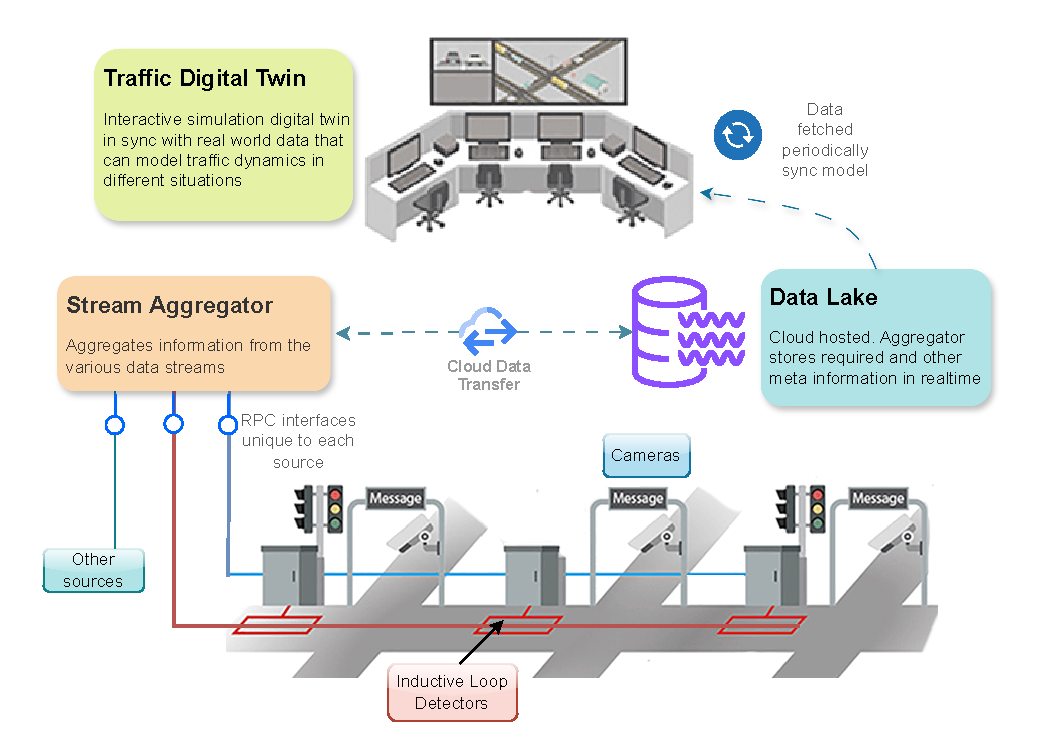
\includegraphics[width=0.77\textwidth]{framework.pdf} % Adjust width as needed
  \caption{Traffic Digital Twin (TDT) data processing}
  \label{fig:framework}
\end{figure*}

\begin{enumerate}[(i)]
    \item Hardware infrastructure should be cheap and easily replaceable.
    \item Easily extendable to use a variety of different sources.
    \item Should work with only absolute traffic counts, no other specific information like direction and vehicle types.
    \item Should work with a medium-frequency update.
\end{enumerate}

There are various possible ways to collect the type of data mentioned. The most reliable would be to install inductive loop detectors embedded in road surfaces at city intersections. Such systems are already available and in use in several major cities. For example, the Sydney Coordinated Adaptive Traffic System (SCATS)\cite{scats} is available in over 180 cities across 28 countries, including New Zealand, Dublin, Shanghai, and Hong Kong \cite{wiki:sydney_traffic_system}. New York City's Adaptive Traffic Control System (ATCS), Adaptive Signal Control Technology (ASCT), SCOOT, and ACS are other such systems that are used to control traffic signal timings and optimize congestion. Such systems can be easily extended to use with our proposed model since we only use absolute traffic volume counts, which such systems are capable of collecting.

Another possible data source can be surveillance cameras assisted with computer vision models\cite{jain2019review}, which is already used in practice at some intersections in Shenzhen, China. Several existing studies\cite{asha2018vehicle} using state-of-the-art object detection models like YOLO\cite{redmon2018yolov3} demonstrate the effectiveness of this method. Such a model-based approach allows for cheap and effective traffic monitoring on top of existing surveillance camera infrastructure. 

Other methods like using GPS-enabled mobile phones\cite{rose2006mobile} to track urban traffic flow, as Google does in its Maps product, and the use of probe vehicles\cite{zhu2012probe}, which are vehicles equipped with detectors that may be taxis or public transport, can also be used to approximate traffic volume based on their data.

We aim for our model to work in conjunction with multiple data streams, as different parts of the road network may be served with different data sources. We want our TDT to integrate with these sources seamlessly, so we need an aggregator of sorts to reconcile the data from the different streams and store them in a data lake. This data can then be used by the TDT model to keep its internal state in sync with real-world data.

The deployed aggregator system will have an RPC and API interface that can be interacted with by the remote sensors and other data sources. Each service can have a separate interface built for interacting with the aggregator service. The aggregator then stores all the data with relevant meta information in a datalake, a centralized repository that allows you to store all your structured and unstructured data. We make use of a datalake as different sources might have additional information apart from just traffic volume counts, and by allowing us to store other complementary information, we leave possible avenues for building up further capabilities in our TDT.

An example representing a simplified view of the aforementioned process is shown in Fig. \ref{fig:framework}.
%!TEX root=./paper.tex
\subsection{\textbf{Model input}}

For each node, a composite feature vector is constructed to encapsulate all pertinent node-related data. This vector is formed by concatenating three distinct feature vectors, each defined as follows:

\subsubsection{Graph embedding generation using Node2Vec:}\label{subsubsec:embd}

To facilitate the model's understanding of spatial relationships among detector nodes within the graph structure, an effective representation of the nodes' neighborhood structure is essential. Node2Vec \cite{node2vec} addresses this need through a feature learning approach that employs second-order biased random walks within a Skip-gram architecture. The process of generating feature vectors involves two pivotal steps:


\begin{enumerate}[(i)]
    \item \textit{Sampling using second-order biased random walks}: Two hyper-parameters, \( p \) and \( q \), are introduced in the context of Node2Vec, where \( p \) controls the likelihood of revisiting nodes in the random walk (termed as the "return" parameter), and \( q \) adjusts the likelihood of exploring nodes further away from the current node (termed as the "in-out" parameter). Let \( l \) denote the fixed length of the simulated random walk starting at node \( u \), with \( c_i \) representing the \( i \)th node in the walk (\( c_0 = u \)). Nodes \( c_i \) are generated according to the following distribution:

    \[
        P(c_i = x \mid c_{i-1} = v) =
        \begin{cases}
        \frac{\pi_{vx}}{Z} & \text{if } (v,x) \in E \\
        0 & \text{otherwise}
        \end{cases}
    \]
    where \( \pi_{vx} \) is the unnormalized transition probability between nodes \( v \) and \( x \), and \( Z \) is the normalizing constant.
    
    For a random walk that has just traversed edge \( (t,v) \) and is currently at node \( v \), the next step involves evaluating transition probabilities \( \pi_{vx} \) for edges \( (v,x) \) leading from \( v \). Here, the transition probability is determined by \( \pi_{vx} = \alpha_{pq}(t,x) \cdot w_{vx} \), where \( \alpha_{pq}(t,x) \) denotes the transition probability adjustment factor defined as:

    \[
        \alpha_{pq}(t,x) = 
        \begin{cases}
        \frac{1}{p}  & \text{if } d_{tx} = 0\\
        1 & \text{if } d_{tx} = 1\\
        \frac{1}{q} & \text{if } d_{tx} = 2
        \end{cases}
    \]
    and \( d_{tx} \) denotes the shortest path distance between nodes \( t \) and \( x \).

    \item \textit{Optimizing objective function using Skip-gram}: Let \( G(V, E) \) be a graph where \( f: V \rightarrow \mathbb{R}^d \) denotes the function mapping each node \( u \) to a \( d \)-dimensional feature representation. Hence, \( f \) forms a matrix of parameters sized \( |V| \times d \). For each node \( u \in V \), let \( N_S(u) \subset V \) represent the \emph{network neighborhood} generated in step (i). The similarity between nodes \( u \) and \( v \) is defined as:

    \[
        P_f(v|u) = \frac{\exp(f(v)^T f(u))}{\sum_{w \in V} \exp(f(w)^T f(u))} \tag{1}
    \]
    For neighborhood \( N_s(v) \) of \( v \), define the probability of the neighborhood of \( u \) as:
    
    \[ P_f(N_s(u)|u) = \prod_{v \in N_s(u)} P_f(v|u) \tag{2} \]

    Further, the global neighborhood likelihood for a given \( f \) can be defined as:
\[ \sum_{u \in V} \log P_f(N_s(u) \mid u) \tag{3} \]
which is the objective function that we want to maximize through the feature representation function \(f\). Hence,
\[ \max_{u \in V} \sum_{u \in V} \log \left( \prod_{v \in N_s(u)} \frac{\exp(f(v)^T f(u))}{\sum_{w \in V} \exp(f(w)^T f(u))} \right) \tag{4} \]

\end{enumerate}

\begin{figure*}[htbp]
  \centering
  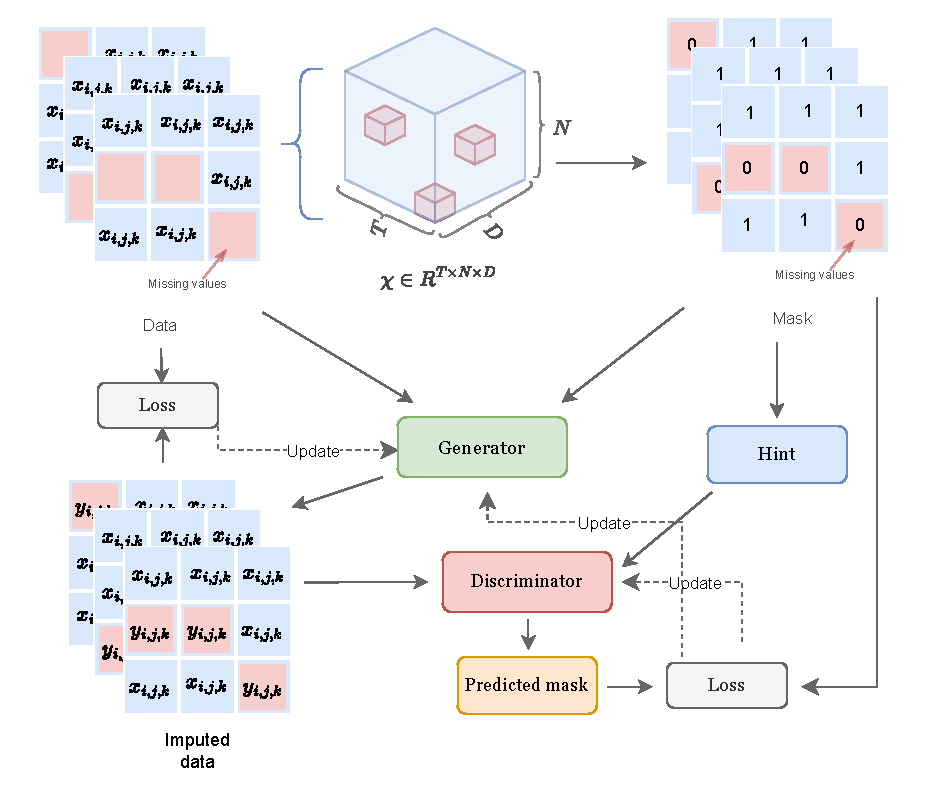
\includegraphics[width=0.85\textwidth]{model.pdf}
  \caption{Model architecture}
  \label{fig:dataset}
\end{figure*}

\subsubsection{Normalizing traffic volume}\label{subsubsec:normal}
The input data should be normalized to increase the training speed and effectiveness. The traffic volume counts at different detectors are normalized as follows:

\[ x_{\text{norm}} = \frac{x - x_{\text{min}}}{x_{\text{max}} - x_{\text{min}}} \]
Thus, \( x_{\text{norm}} \) is in the range \([0,1]\) after normalization.
This same approach is used for other continuous or discrete single-valued features.

\subsubsection{Word2Vec encoding of other exogenous variables:}\label{subsubsec:encode}
The Skip-gram architecture, a prominent model in natural language processing~\cite{skipgram}, operates under the Word2Vec framework~\cite{word2vec}. Its primary objective is to predict surrounding context words based on a given target word. By doing so, Skip-gram effectively learns to encode semantic meanings of words by maximizing the conditional probability of context words given the target word. This objective function is mathematically formulated as:
\[
J_\theta = \frac{1}{T}\sum^{T}_{t=1}\sum_{-n\leq j \leq n, j \neq 0}\log p\left(w_{j+1} \mid w_{t}\right)
\]

where \( w_t \) represents the target word at position \( t \), \( c \) is the size of the context window, and \( T \) is the total number of words in the corpus.

In our methodology, we employ \textit{Word2Vec} \cite{word2vec} to encode various exogenous variables such as weather conditions, road types, and other potentially relevant factors into feature vectors for the model input. This enhancement aims to augment the model's effectiveness by capturing semantic relationships between these variables and the observed traffic patterns. Importantly, our approach is designed to accommodate future extensions, allowing for the inclusion of additional relevant features as they are identified and integrated into the model input.

Concatenating the feature vectors obtained from Sections~\ref{subsubsec:embd} to \ref{subsubsec:encode}, we derive the final input vector for our model. Extending upon the notation introduced in Section~\ref{sec:problem-for}, for $N$ nodes, we define $\mathbf{x}_i^t$, the feature vector of node $i$ at time $t$. Assuming the use of \textit{Node2Vec} as described in (i) to generate $R^{D_g}$-dimensional graph embeddings $g_i$ for each node $i$, and normalizing $n$ single-dimensional real-valued features $(r_1, r_2, \ldots, r_n)$ as outlined in (ii) to $(r_1^{\text{norm}}, r_2^{\text{norm}}, \ldots, r_n^{\text{norm}})$, resulting in a $D_n = n$ dimensional vector $h_i^t$. Additionally, leveraging \textit{Word2Vec} to produce $d_w$ dimensional vectors for $m$ semantic "words" related to each node, we obtain a $R^{m \times d_w}$-dimensional vector flattened and represented as $k_i^t \in R^{D_w}$, where $D_w = m \times d_w$.

Finally, by concatenating the feature vectors described in Section~\ref{subsubsec:embd} -~\ref{subsubsec:encode}, we obtain the feature vector of node $i$ at time $t$:
\[
\mathbf{x}_i^t = ( g_i || h_i^t || k_i^t ) \in \mathbb{R}^D
\]
where $D = D_g + D_n + D_w$. Thus, leveraging the methodologies outlined in Eq~(\ref{eq:X}) and (\ref{eq:chi}), across $T$ consecutive time steps and for $N$ nodes, we construct the final feature vector $\mathbf{\chi} \in \mathbb{R}^{T \times N \times D}$. Depending on the specific task, additional inputs such as a binary matrix $M$ representing missing and known values are included. %Further implementation details are discussed in the experiments section.

%!TEX root=./paper.tex
\subsection{\textbf{Physics Informed Deep Learning}}

Physics-informed deep learning (PIDL) represents a distinct approach within deep learning (DL), where a neural network is trained to tackle learning tasks while adhering to the principles of physics. By integrating fundamental physical laws as prior knowledge, the resulting neural network serves as a data-efficient approximator, adept at processing input data and delivering accurate predictions.

In situations where systems are required to adhere to the physical laws, PIDL is especially useful as it biases the model to follow the physics models; this allows the model to generate more accurate results, specially GANs, as this eliminates several possible predicted distributions that are not viable do to not adhering to the physical laws of the system.

In our situation, specifically with problem 3. of Traffic assignment on edge addition/removal, where we have to predict the changed volume counts on the same timestep but with modified topology, it is imperative, according to the \textit{conservation law} of traffic, that in such a case that the total volume of traffic in a large enough region prior to and after redistribution will be same.

Formally, for a particular fixed time, let \( G(V, E) \) be the original graph, and \( G'(V', E') \) be the graph obtained by adding or removing an edge \( e \). Similarly, \( c_i \) represents the traffic volume at detector \( i \) in \( G \) for \( i = 1 \) to \( N = |V| \), and \( c_i' \) represents the traffic volume at detector \( i \) in \( G' \) for \( i = 1 \) to \( N' = |V'| \). Then from \textit{conservation law}:
\begin{equation}
    C = \sum_{i=1}^{N} c_i = C' = \sum_{i=1}^{N'} c'_i \tag{5}
\end{equation}

In order to bias the model for conservation as described in Eq. (3), it needs to be integrated into the learning process of the PIDL network. The simplest way to do it is to define it as an additional term to the loss used to update the model, basically penalizing the model heavily for predictions that do not conform to the physical constraints. With traffic volumes \(c_i\) along with other graph information as training input, we establish two different measures for the discriminator to evaluate generator output:
\begin{enumerate}
    \item \textbf{\( \mathcal{L}_{DL} \)}: Denoting the conventional discriminator loss defined as:
    \[ \mathcal{L}_{DL} = \mathbb{E}_{x \sim P_{\text{data}}}[D(x)] - \mathbb{E}_{z \sim P_z}[D(G(z))] \]

    \item \textbf{\( \mathcal{L}_{PHY} \)}: Denoting the conservation loss. As defined in Eq. (3), for a given mask \( M \), let \( S \) be the set of detectors such that \( M(i) = 0 \), specifically \( S = \{i \mid M(i) = 0\} \). Then let \( C_0 \) be the sum of masked traffic volume counts, i.e., \( C_0 = \sum_{i \in S} c_i \), and \( Y = \{c'_i \mid i \in S\} \) be the generator output. Then define:
    \[ \mathcal{L}_{PHY} = (C_0 - \sum_{i \in S} c'_i)^2 \]
\end{enumerate}
In order to control the dominance of the different components of the loss function, we introduce two new hyperparameters, \( \mu \) and \( \lambda \), to adjust the weights of \( \mathcal{L}_{DL} \) and \( \mathcal{L}_{PH} \) respectively. Thus, the final loss function can be defined as:

\[ \mathcal{L} = \mu \cdot \mathcal{L}_{DL} + \lambda \cdot \mathcal{L}_{PHY} \]

In conclusion, by leveraging hyperparameters, we can fine-tune the model's balance between different objectives. Biasing the discriminator to respect physical laws allows the generator to better capture the underlying patterns in the data, a capability we found useful in our experiments, as we describe ahead.
%!TEX root=./paper.tex
\subsection{\name: Traffic Model}

In this section, we present the architecture of our \name model, which is inspired from architectures of Generative Adversarial Imputation Nets (GAIN)\cite{gain} and Wasserstein Generative Adversarial Network (WGAN)\cite{wgan}. GAIN is a new and popular type of conditional GAN that has been applied to a variety of missing value imputation tasks on different datasets with favorable results. WGAN is an improvement over traditional GANs proposed by M. Arjovsky et al., that is designed to improve training stability by focusing on using Wasserstein distance metric instead of the traditional Jensen-Shannon divergence, along with some other architecture changes like gradient clipping, removal of sigmoid, etc., that have been shown to result in more reliable convergence and better quality samples.

\subsubsection{\textit{Generator:}}

The generator \( G \) accepts inputs of observed data, with missing values, denoted by \( \mathbf{X} \), the binary mask vector \( \mathbf{M} \) which indicates what are the missing values, and a noise vector denoted by \( \mathbf{Z} \). It produces imputed data \( \mathbf{X}_g \), representing a vector of imputations, which is then projected to form the complete imputed output \( \mathbf{Y}_0 \). 

Formally, the output of the generator \( G \) can be denoted as: 
\[ \mathbf{X}_g = G(\mathbf{X}, \mathbf{M}, (\mathbf{1}-\mathbf{M}) \odot \mathbf{Z}) \]

where \( \odot \) denotes the Hadamard product or the element-wise multiplication and \( \mathbf{Z} \) is the \( d \)-dimensional noise vector. \( \mathbf{X}_g \) represents the missing values which are then filled back in \( \mathbf{X} \) as per the mask \( \mathbf{M} \), and this makes the final generator output that is then passed off to the discriminator to judge.

\subsubsection{\textit{Discriminator:}}

Similar to the discriminator in traditional GANs, we also use another model called the Discriminator, denoted by \( D \), that acts as an adversary to the Generator \( G \) and trains it. The discriminator \( D \) defined in the original GAIN implementation as \( D : \mathbf{\chi} \rightarrow [0,1]^d \), outputs a binary vector instead of a single real value, which denotes what components of the generator input are real (observed) and what are fake (imputed). 

So, in contrast to the traditional discriminator as used in GANs, which predicts whether the generated result is entirely fake or real, the discriminator in GAIN predicts what components are real or fake. And the loss which is then used in SGD is the mean of losses for individual components.

\subsubsection{\textit{Hint}}
GAIN introduces a new concept called the hint mechanism, represented by a random variable \( \mathbf{H} \) taking values in a space \( \mathcal{H} \). The aim of this hint mechanism is to provide additional missing information to the discriminator about the mask. The following proposition was introduced and proved in the GAIN\cite{gain} original paper:

\begin{mdframed}[linewidth=0.5pt]
\textit{
\newtheorem{proposition}{Proposition}
\begin{proposition} \label{prop:nonunique}
    There exist distributions of \( \mathbf{X} \), \( \mathbf{M} \), and \( \mathbf{H} \) for which solutions to \( \hat{p}(\mathbf{x} | \mathbf{h}, m_i = t) = \hat{p}(\mathbf{x} | \mathbf{h}) \) for each \( i \in \{1, \ldots, d\} \), \( \mathbf{x} \in \mathcal{X} \), and \( \mathbf{h} \in \mathcal{H} \) such that \( p_h(\mathbf{h} | m_i = t) > 0 \) are not unique under the optimality criterion of GAN.
\end{proposition}
}
\end{mdframed}

This means that there may exist several possible distributions that \( G \) may generate that may seem valid to \( D \), so \( \mathbf{H} \) must provide enough information to uniquely identify the correct representation of the underlying data, which is what the hint mechanism aims to do.

The hint mechanism depends on the binary mask vector \( \mathbf{M} \), and for each imputed sample \( (\hat{\mathbf{x}}, \mathbf{m}) \), we draw \( \mathbf{h} \) from the distribution \( \mathbf{H} | \mathbf{M} = \mathbf{m} \). We then add \( \mathbf{h} \) as an extra input to the discriminator, resulting in a function \( D: \mathcal{X} \times \mathcal{H} \rightarrow [0, 1]^d \), where each component of \( D(\hat{\mathbf{x}}, \mathbf{h}) \) represents the probability that the corresponding component of \( \hat{\mathbf{x}} \) was observed given \( \hat{\mathbf{X}} = \hat{\mathbf{x}} \) and \( \mathbf{H} = \mathbf{h} \).
By varying how \( \mathbf{H} \) is defined, we control the level of information it provides about \( \mathbf{M} \).

\textcolor{gray!80}{\vrule width 0.95\columnwidth height 0.001pt depth 0pt \relax}

\vspace{1ex}

Finally, we take inspiration from the architecture of WGAN and incorporate some of those changes in our model. Traditional GANs suffer from training instability and model collapse, i.e., inability to learn the diverse representations and only generating repetitive samples. Wasserstein GAN (WGAN) proposed by M Arjovsky et. al, solves these problems and we highlight some of the architectural changes we made to GAIN based on WGAN in the following paragraphs.

In traditional GAN the generator and discriminator are trained using the following loss functions:
\[
\mathcal{L}_{\text{GAN}}^G = \log(1 - D(G(z)))
\]
\[
\mathcal{L}_{\text{GAN}}^D = -\log(D(x)) - \log(1 - D(G(z)))
\]

whereas in WGANs, we remove the logarithms and use Wasserstein distance for loss instead.
\[
\mathcal{L}_{\text{WGAN}}^G = -D(G(z))
\]
\[
\mathcal{L}_{\text{WGAN}}^D = D(G(z)) - D(x)
\]

Another change in WGANs, that we incorporate in GAIN is the absence of a sigmoid activation function in the discriminator's output layer, unlike in traditional GANs. This alteration enables the discriminator to output unbounded real-valued scores instead of probabilities. Additionally, WGANs incorporate gradient clipping as a regularization technique to enhance training stability. Gradient clipping involves setting a threshold value for the gradients, and if they exceed this threshold, they are scaled down to ensure that their magnitude does not surpass it. This approach helps stabilize the training process and mitigates issues such as exploding gradients.

%!TEX root=./paper.tex
\section{Experiments}\label{sec:experiments}
In this section, we present the experimental results of our model, detailing the parameters necessary to replicate these outcomes. Additionally, we provide a description of the baseline models used for comparison, along with their respective parameters.

\subsection{Dataset Description}

We utilize real-world traffic volume data from Dublin city streets, collected using the SCATS (Sydney Coordinated Adaptive Traffic System) over a three-month period. SCATS is employed in Dublin as an adaptive urban traffic management system that synchronizes traffic signals and optimizes traffic flow across the entire city.

The dataset comprises traffic volumes from 825 sensors located at key intersections in Dublin city, sampled hourly from October 1, 2023, to December 31, 2023. This dataset includes the latitudinal and longitudinal geographical coordinates along with the timestamped total traffic volume detected by each sensor within each one-hour period.

Weather data, used in conjunction with the traffic data, is sourced from the official website of Met Éireann, the state meteorological service of Ireland. This data includes hourly information on weather phenomena such as air temperature, relative humidity, visibility, and precipitation amount, collected from three weather stations within the city of Dublin.

We also verify the model for task (iii) using the SUMO~\cite{sumo} TAPASCologne scenario~\cite{tapas}, which simulates the traffic dynamics of Cologne, Germany, over a day. This scenario is publicly available on the official SUMO website and was created using mobility demand data based on citizens' travel habits and information about the local infrastructure. Due to the manual nature of this testing, we conduct a limited number of tests where we alter an edge, process the simulation based on the default minimal travel time routing before and after the change, and observe the deviation between the simulation and our results.

\begin{figure}[htbp]
  \centering
  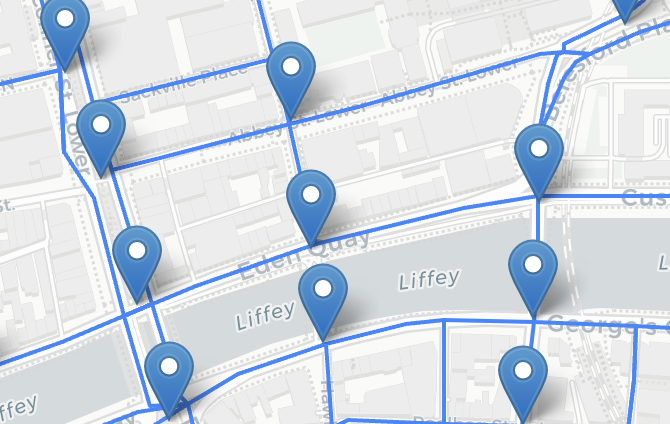
\includegraphics[width=0.5\textwidth]{dataset.png}
  \caption{Snapshot of sensor locations plotted along with road network from Overpass API}
  \label{fig:dataset}
\end{figure}


\subsection{Model Parameters}

For all experiments, we set hyperparameters \(T = 3\), representing the number of consecutive timesteps to consider for prediction and imputation tasks. For all tasks, we optimize the model input by assuming the locality of traffic within such a timespan and that any changes to a particular node are only dependent on nodes "close" to it. During training, we train on subgraphs consisting of node clusters instead of the entire graph at once. Specifically, a subgraph is generated by choosing a node \(u\) at random and then selecting all nodes that are at a distance less than \(\sigma\) to it. Formally, for \(G(V, E)\), the subgraph is defined as \(G_{\text{sub}} = G\{v \in V \mid \text{dist}(u, v) < \sigma\}\). For our experiments, we set \(\sigma\) to \(2.5\ km\), which is reasonable as clusters usually contain 20 to 30 nodes within this range.

After sampling, as stated, we use an 80-20 test-train split, meaning the model is trained on 80\% of the samples, and performance is verified on new unseen data comprising 20\% of the samples. The data is then modified based on the task at hand. For imputation, we followed the MCAR (Missing Completely at Random) distribution and randomly masked values both spatially and temporally, based on a parameter defined as the miss rate. We tested our model on miss rates of 10\%, 20\%, 30\%, and 40\%. For prediction, we use the full data of three timesteps to predict the fourth step by masking the values along the last timestep dimension. For the re-assignment task, i.e., task (iii), we only consider one timestep and re-assign values for that same timestep but with modified spatial geometry.

\subsection{Baselines}

We compare our \name\ model with several existing approaches across different domains, including various mathematical analysis and deep learning techniques that are commonly used for these tasks.

For imputation, one of the simplest approaches is \textit{KNN}. For prediction, \textit{ARIMA} (AutoRegressive Integrated Moving Average) \cite{arima} is employed. Matrix factorization methods such as \textit{TRMF} (Temporal Regularized Matrix Factorization) \cite{trmf} use latent factors for predictions, with \textit{BTRMF} (Bayesian Temporal Regularized Matrix Factorization) extending TRMF within a Bayesian framework. For both TRMF and BTRMF, we use a rank of 10, 1000 burn-in iterations, and 200 Gibbs iterations.

\textit{LRTC-TNN} (Low-Rank Tensor Completion with Truncated Nuclear Norm) \cite{lrtc} is a method for tensor completion, using parameters $\rho = 1e-5$, $\theta = 0.25$, and $\epsilon = 1e-4$. \textit{BGCP} (Bayesian Gaussian Process Factorization) utilizes Bayesian inference. For BGCP, we use similar burn-in and Gibbs iterations and set the rank to 30. It is important to note that these model baselines are applicable only to task (i) and task (ii), and not to task (iii) since they were not designed for that task.

Additionally, we employed deep learning methods. For imputation, we used the \textit{Denoising AutoEncoder} (DAE) \cite{dae} model, which is effective in learning meaningful representations of the data while handling missing values. For prediction tasks, we utilized an \textit{LSTM} (Long Short-Term Memory) \cite{lstm} model, as LSTM networks are well-suited for capturing temporal dependencies in sequential data.


\subsection{Evaluation metrics}

To evaluate the performance of the different methods and compare them, we use RMSE (Root Mean Squared Error) and MAPE (Mean Absolute Percentage Error). These metrics are defined as follows:

\[
\text{RMSE} = \sqrt{\frac{1}{n} \sum_{i=1}^{n} (y_i - \hat{y}_i)^2}
\]

\[
\text{MAPE} = \frac{1}{n} \sum_{i=1}^{n} \left| \frac{y_i - \hat{y}_i}{y_i} \right| \times 100\%
\]

where \( y_i \) represents the true value, \( \hat{y}_i \) represents the predicted value, and \( n \) is the number of samples.
%!TEX root=./paper.tex
\subsection{Results}

\begin{figure*}[]
  \centering
  \begin{subfigure}[b]{0.9\textwidth}
      \centering
      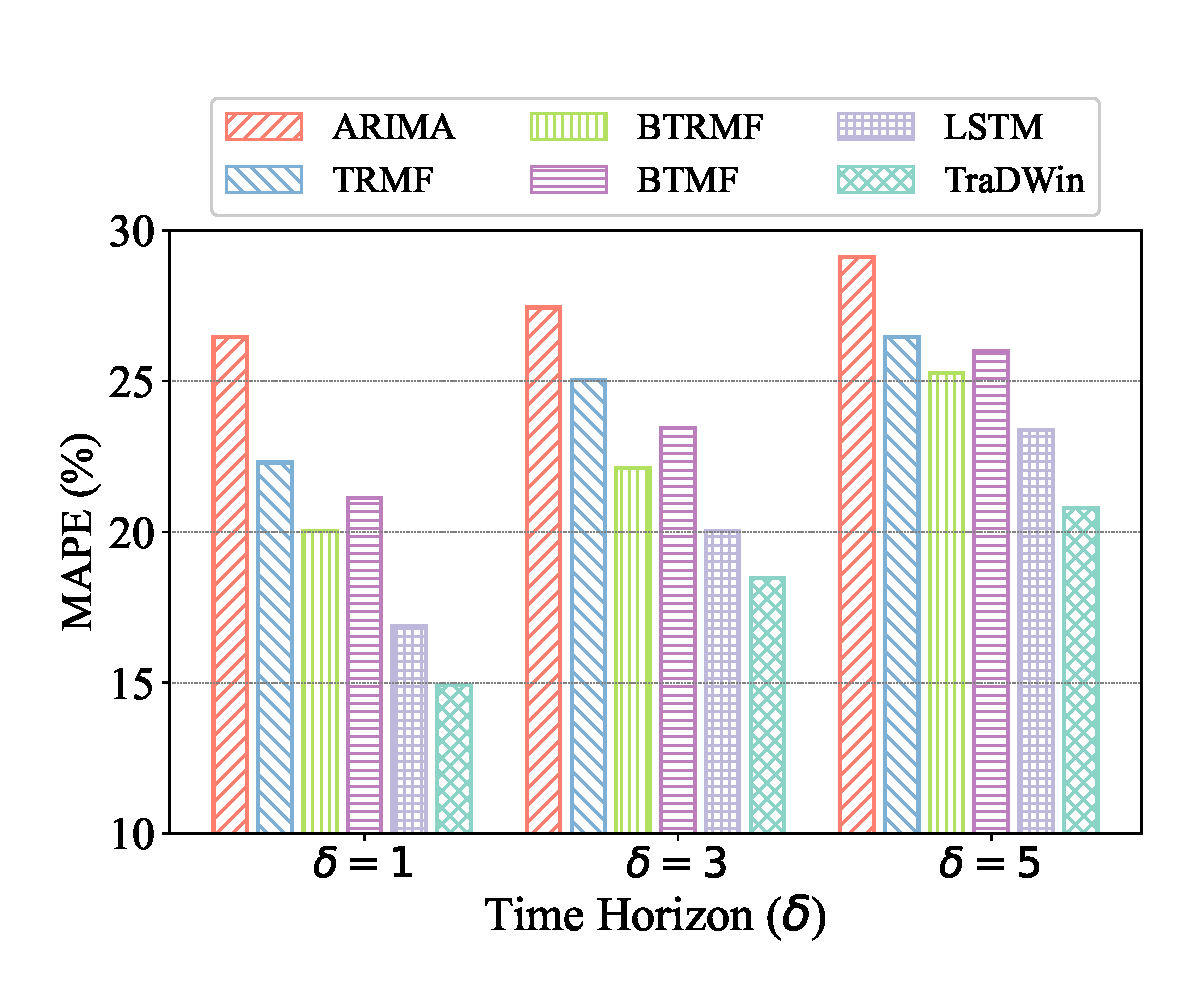
\includegraphics[width=\textwidth]{mape_pred.eps}
      \caption{MAPE on prediction task for different deltas}
      \label{fig:mape_pred}
  \end{subfigure}
  
  \begin{subfigure}[b]{0.9\textwidth}
      \centering
      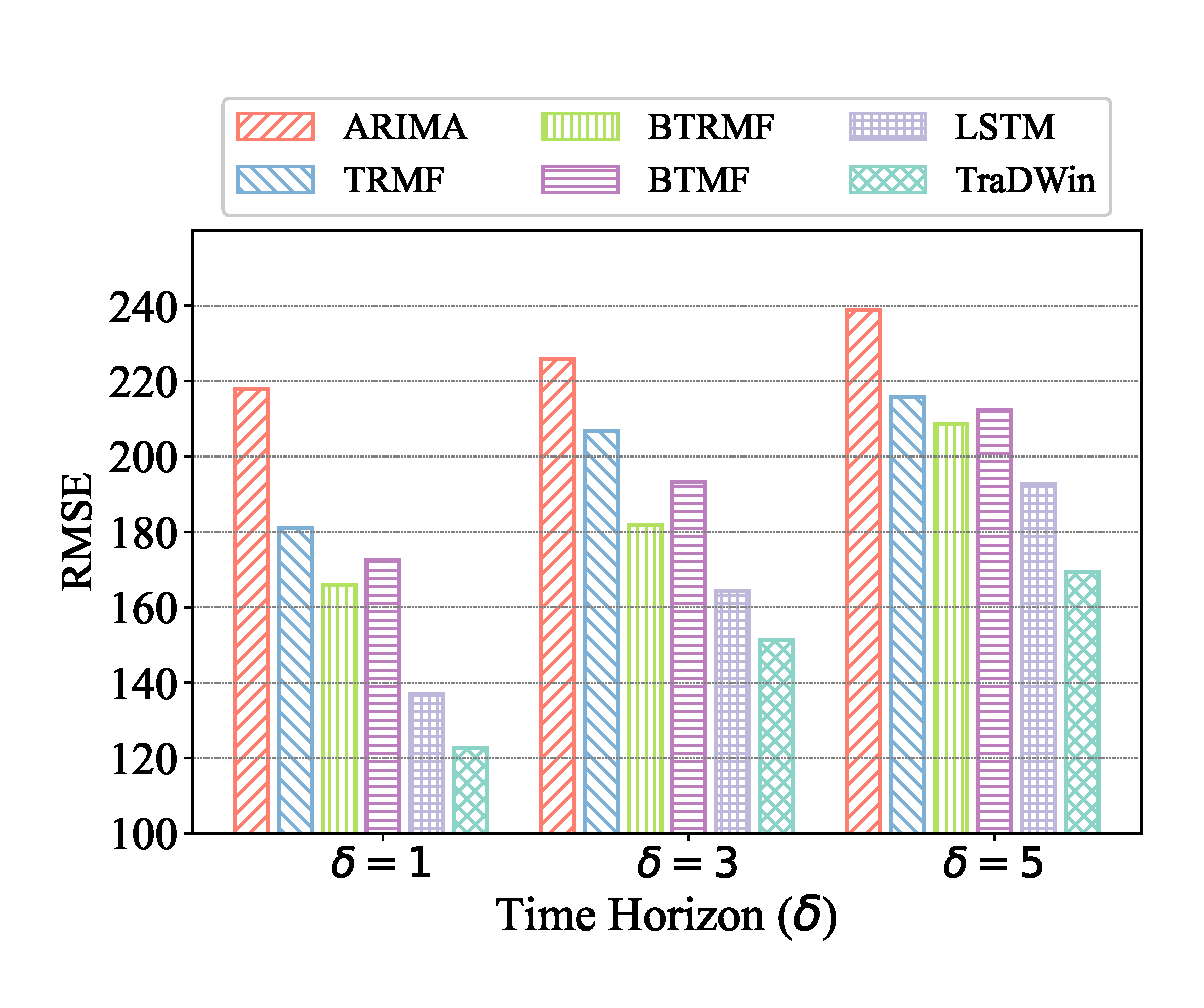
\includegraphics[width=\textwidth]{rmse_pred.eps}
      \caption{RMSE on prediction task for different deltas}
      \label{fig:rmse_pred}
  \end{subfigure}
  
  \caption{Performance metrics on prediction task for different deltas (timesteps to predict ahead)}
  \label{fig:pred_metrics}
\end{figure*}

We evaluate the performance of our model on various tasks and compare it with other popular models in the domain. For the prediction task, we test the models for predicting traffic volumes at the next timestep (\(\delta = 1\)), at the third timestep (\(\delta = 3\)), and at the fifth timestep in the future (\(\delta = 5\)). This scenario requires a mask consisting of all the \(T_{n+1}\) values missing, i.e., 0, for the next timestep prediction. We similarly prepare a mask for other time horizons, treating prediction as a strict MNAR (Missing Not At Random) subcategory of imputation.

The MAPE and RMSE plots of prediction tasks across different horizons are shown in Fig. \ref{fig:mape_pred} and Fig. \ref{fig:rmse_pred}, respectively. We observe that generally, as the time horizon \(\delta\) increases, both metrics worsen, with MAPE falling 5-10\% from \(\delta=1\) to \(\delta=3\). This indicates a stronger short-term accuracy but some challenges with long-term prediction across all models. This trend is common in time-series forecasting, where predictive accuracy decreases as the prediction horizon extends. The primary reasons for this decline include the increasing uncertainty and the influence of unpredictable external factors, such as accidents or weather changes.

ARIMA performs the worst, which is expected as it is the simplest of the mathematical models among the baselines we consider. Other matrix factorization and Bayesian models like TRMF, BTRMF, and BTMF perform better but, being strictly mathematical models, they (i) fail to capture the intricate traffic dynamics that a deep learning model can and (ii) use only the time-series traffic data and not the graph topology and external factors, such as weather, that our model considers. LSTMs perform close but slightly worse (by 2-3%), likely due to the lack of knowledge of graph topology that our model incorporates through Node2Vec.

Overall, our \name\ model performs significantly better than most models, scoring roughly 3 to 7 percentage points better than the baselines.

\begin{figure*}[]
\centering
\begin{subfigure}{0.5\textwidth}
  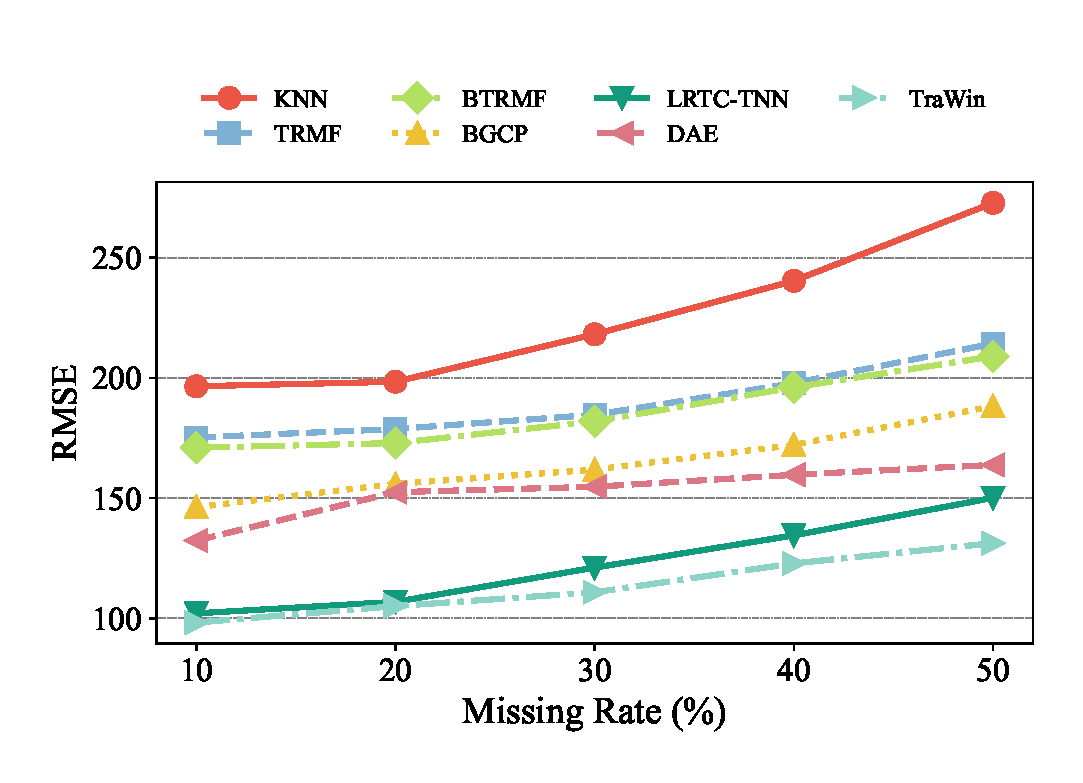
\includegraphics[width=\linewidth]{rmse_imput.eps}
  \caption{RMSE of different models on imputation task}
  \label{fig:mape_imput}
\end{subfigure}%
\begin{subfigure}{0.5\textwidth}
  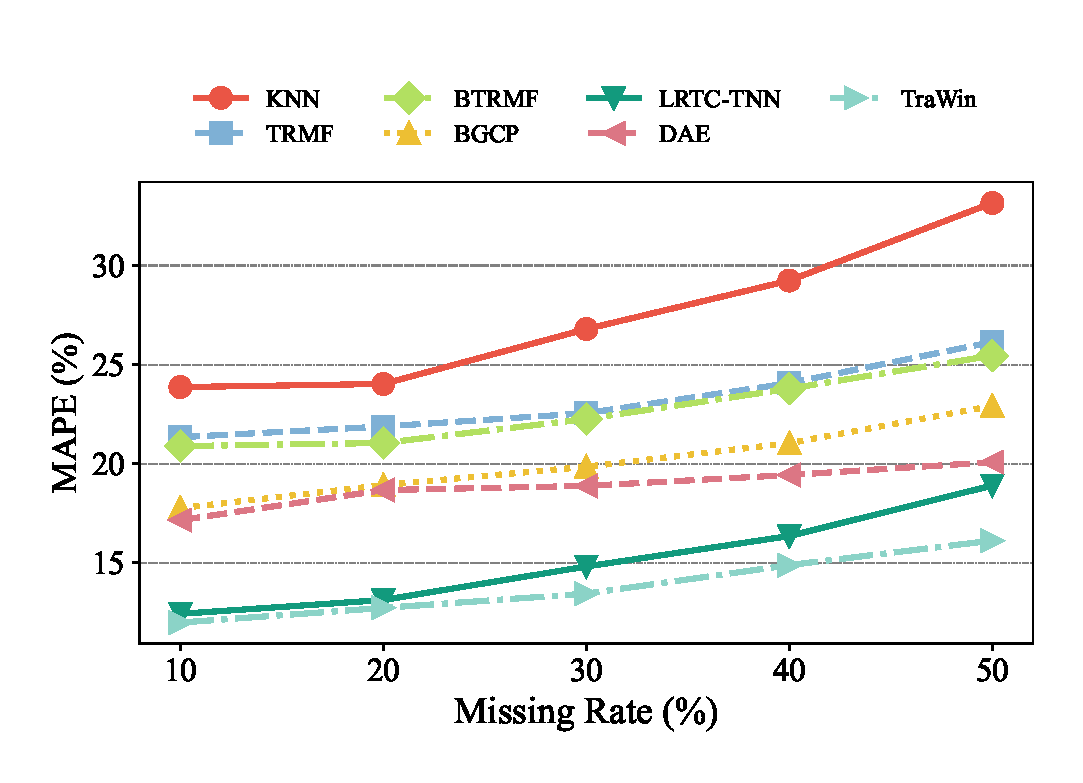
\includegraphics[width=\linewidth]{mape_imput.eps}
  \caption{MAPE of different models on imputation task}
  \label{fig:rmse_imput}
\end{subfigure}
\caption{Imputation comparison for different missing rates}
\label{fig:imput}
\end{figure*}

We evaluate performance on the imputation task. For this task, we consider the MCAR (Missing Completely At Random) distribution and compare the models at five missing rates of $10\%$, $20\%$, $30\%$, $40\%$, and $50\%$. The performance of different models, measured using MAPE and RMSE, is shown in Fig. \ref{fig:imput}. Conventional methods like KNN perform poorly compared to more specialized approaches, as expected, since KNN is insufficient to capture intricate traffic dynamics. Matrix factorization and Bayesian methods, such as TRMF, BTRMF, and BGCP, work slightly better, with deep learning methods like DAE performing ahead. However, since they deal only with traffic data time series without topology information, their performance is 8-13\% worse than our model. Tensor completion-based models like LRTC-TNN are close to our \name\ for low missing rates but do not scale as well with increasing missing rates. This could be because too much data is lost for reliable tensor completion, which a deep learning model can handle due to its ability to learn complex data relationships and incorporate graph topology and other external factors. It is also worth noting that LRTC-TNN, an MCAR imputer, is not applicable to task (iii) and is not generalized enough for our use case. For all models, the accuracy of imputations decreases with higher missing rates due to the reduced amount of contextual information available, a common challenge in data imputation. Overall, our \name\ scales well with more missing data and performs significantly (5-7\%) better than the compared baselines.

We observe that \name\ performs better on task (ii) than on task (i) by around 4\%. One primary reason for this could be that GAIN, originally designed for MCAR imputation, does not generalize well to MNAR imputation scenarios. Another possible reason could be the subgraph-based computation method we use, where nodes at the corners of the subgraph lack adequate spatial and temporal information about their neighbors. Overall, our model performs reasonably and delivers comparable results as a generalized model on both tasks.

For the re-assignment task, which is a new task addressed in our paper and not commonly seen in contemporary literature, we train the model for MNAR imputation scenarios with the central node cluster missing. This training effectively teaches the model to assign traffic to node clusters based on neighbor node information. To elaborate, for a modified edge, nodes around the edge, based on a distance threshold, are masked (i.e., marked missing). The training input includes features for the neighbors of the cluster (nodes not masked out), graph embeddings for the masked nodes (not the traffic volume as that is marked missing), and the total volume of traffic for the masked-out nodes. The task is to assign traffic volumes to the masked-out nodes and compare them against the original values. The model learns "traffic assignment" since real-world labeled data for traffic state before and after modification of edges is unavailable. Based on this training task, we achieve a MAPE of $13.47\%$ and RMSE of $109.90$. The other baselines considered for prediction and imputation are not applicable without changes to their model architecture, so there is no comparison with contemporary models.

The de-facto way to solve this problem, as observed in our literature review, has been through simulations like SUMO\cite{sumo} and Vissim\cite{vissim}. Using SUMO, we also compare and test our model on the TAPASCologne scenario. We train using the same approach as for the Dublin SCATS dataset but test against the simulation results after modifying the said edge. This is not possible for the Dublin dataset since detailed origin-destination pair data is unavailable. The results of our model on this task are shown in Table \ref{reassign_table}. We observe that the model achieves a MAPE of $13.47\%$ on the Dublin SCATS dataset and $15.06\%$ on the TAPASCologne scenario, demonstrating the model's reasonable accuracy in solving the traffic assignment problem on node clusters. Furthermore, we evaluate how our model's performance scales with the number of modifications, i.e., how much we can alter the original graph while keeping the model viable for re-assignment. Fig. \ref{fig:edge_modif} shows a comparison of MAPE and RMSE with the number of edges modified. Performance declines steadily from $13.47\%$ at one change to $31.91\%$ at five changes, indicating that more graph alterations lead to a significant performance drop, especially after three modifications. A possible reason for this could be the mass masking strategy used to train the model for task (iii), where masking too many neighboring nodes leads to a large loss of contextual information that graph representation knowledge cannot fully compensate.


\begin{figure}[t]
  \centering
  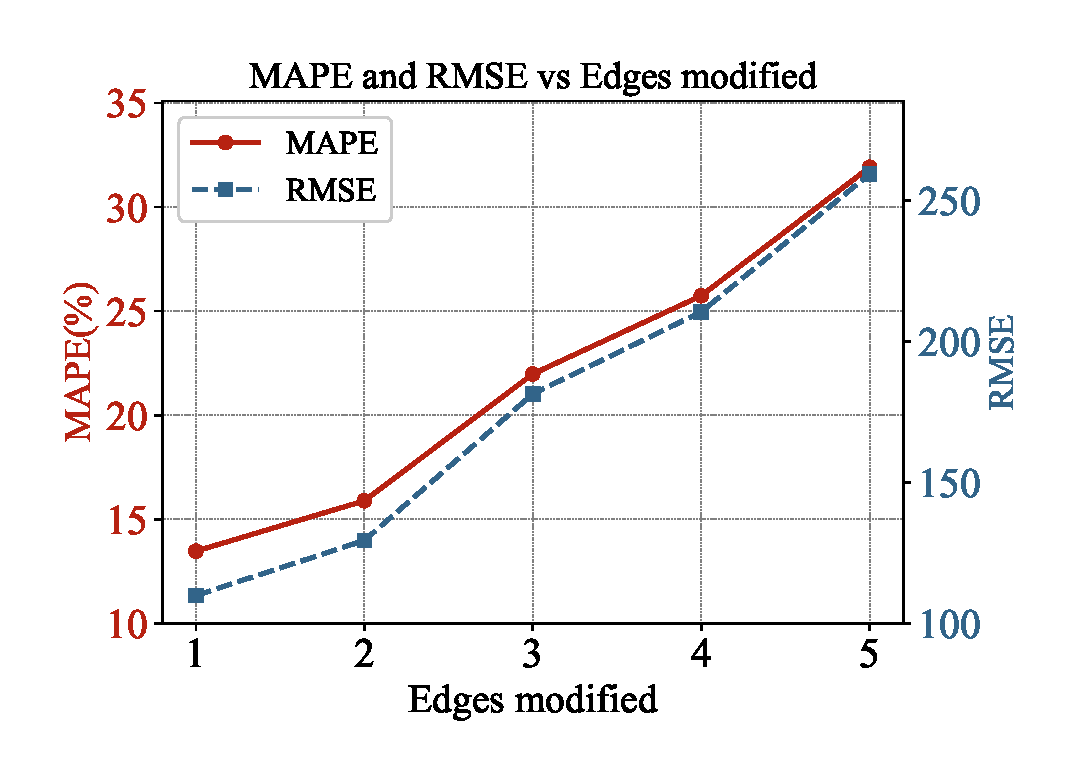
\includegraphics[width=\linewidth]{modif.eps}
  \caption{MAPE and RMSE on re-assignment task vs number of edges modified}
  \label{fig:edge_modif}
\end{figure}

We evaluate performance on the imputation task. For this task, we consider the MCAR (Missing Completely At Random) distribution and compare the models at five missing rates of $10\%$, $20\%$, $30\%$, $40\%$, and $50\%$. The performance of different models, measured using MAPE and RMSE, is shown in Fig. \ref{fig:imput}. Conventional methods like KNN perform poorly compared to more specialized approaches, as expected, since KNN is insufficient to capture intricate traffic dynamics. Matrix factorization and Bayesian methods, such as TRMF, BTRMF, and BGCP, work slightly better, with deep learning methods like DAE performing ahead. However, since they deal only with traffic data time series without topology information, their performance is 8-13\% worse than our model. Tensor completion-based models like LRTC-TNN are close to our \name\ for low missing rates but do not scale as well with increasing missing rates. This could be because too much data is lost for reliable tensor completion, which a deep learning model can handle due to its ability to learn complex data relationships and incorporate graph topology and other external factors. It is also worth noting that LRTC-TNN, an MCAR imputer, is not applicable to task (iii) and is not generalized enough for our use case. For all models, the accuracy of imputations decreases with higher missing rates due to the reduced amount of contextual information available, a common challenge in data imputation. Overall, our \name\ scales well with more missing data and performs significantly (5-7\%) better than the compared baselines.

We observe that \name\ performs better on task (ii) than on task (i) by around 4\%. One primary reason for this could be that GAIN, originally designed for MCAR imputation, does not generalize well to MNAR imputation scenarios. Another possible reason could be the subgraph-based computation method we use, where nodes at the corners of the subgraph lack adequate spatial and temporal information about their neighbors. Overall, our model performs reasonably and delivers comparable results as a generalized model on both tasks.

For the re-assignment task, which is a new task addressed in our paper and not commonly seen in contemporary literature, we train the model for MNAR imputation scenarios with the central node cluster missing. This training effectively teaches the model to assign traffic to node clusters based on neighbor node information. To elaborate, for a modified edge, nodes around the edge, based on a distance threshold, are masked (i.e., marked missing). The training input includes features for the neighbors of the cluster (nodes not masked out), graph embeddings for the masked nodes (not the traffic volume as that is marked missing), and the total volume of traffic for the masked-out nodes. The task is to assign traffic volumes to the masked-out nodes and compare them against the original values. The model learns "traffic assignment" since real-world labeled data for traffic state before and after modification of edges is unavailable. Based on this training task, we achieve a MAPE of $13.47\%$ and RMSE of $109.90$. The other baselines considered for prediction and imputation are not applicable without changes to their model architecture, so there is no comparison with contemporary models.

The de-facto way to solve this problem, as observed in our literature review, has been through simulations like SUMO\cite{sumo} and Vissim\cite{vissim}. Using SUMO, we also compare and test our model on the TAPASCologne scenario. We train using the same approach as for the Dublin SCATS dataset but test against the simulation results after modifying the said edge. This is not possible for the Dublin dataset since detailed origin-destination pair data is unavailable. The results of our model on this task are shown in Table \ref{reassign_table}. We observe that the model achieves a MAPE of $13.47\%$ on the Dublin SCATS dataset and $15.06\%$ on the TAPASCologne scenario, demonstrating the model's reasonable accuracy in solving the traffic assignment problem on node clusters. Furthermore, we evaluate how our model's performance scales with the number of modifications, i.e., how much we can alter the original graph while keeping the model viable for re-assignment. Fig. \ref{fig:edge_modif} shows a comparison of MAPE and RMSE with the number of edges modified. Performance declines steadily from $13.47\%$ at one change to $31.91\%$ at five changes, indicating that more graph alterations lead to a significant performance drop, especially after three modifications. A possible reason for this could be the mass masking strategy used to train the model for task (iii), where masking too many neighboring nodes leads to a large loss of contextual information that graph representation knowledge cannot fully compensate.

We evaluate performance on the imputation task. For this task, we consider the MCAR (Missing Completely At Random) distribution and compare the models at five missing rates of $10\%$, $20\%$, $30\%$, $40\%$, and $50\%$. The performance of different models, measured using MAPE and RMSE, is shown in Fig. \ref{fig:imput}. Conventional methods like KNN perform poorly compared to more specialized approaches, as expected, since KNN is insufficient to capture intricate traffic dynamics. Matrix factorization and Bayesian methods, such as TRMF, BTRMF, and BGCP, work slightly better, with deep learning methods like DAE performing ahead. However, since they deal only with traffic data time series without topology information, their performance is 8-13\% worse than our model. Tensor completion-based models like LRTC-TNN are close to our \name\ for low missing rates but do not scale as well with increasing missing rates. This could be because too much data is lost for reliable tensor completion, which a deep learning model can handle due to its ability to learn complex data relationships and incorporate graph topology and other external factors. It is also worth noting that LRTC-TNN, an MCAR imputer, is not applicable to task (iii) and is not generalized enough for our use case. For all models, the accuracy of imputations decreases with higher missing rates due to the reduced amount of contextual information available, a common challenge in data imputation. Overall, our \name\ scales well with more missing data and performs significantly (5-7\%) better than the compared baselines.

We observe that \name\ performs better on task (ii) than on task (i) by around 4\%. One primary reason for this could be that GAIN, originally designed for MCAR imputation, does not generalize well to MNAR imputation scenarios. Another possible reason could be the subgraph-based computation method we use, where nodes at the corners of the subgraph lack adequate spatial and temporal information about their neighbors. Overall, our model performs reasonably and delivers comparable results as a generalized model on both tasks.

For the re-assignment task, which is a new task addressed in our paper and not commonly seen in contemporary literature, we train the model for MNAR imputation scenarios with the central node cluster missing. This training effectively teaches the model to assign traffic to node clusters based on neighbor node information. To elaborate, for a modified edge, nodes around the edge, based on a distance threshold, are masked (i.e., marked missing). The training input includes features for the neighbors of the cluster (nodes not masked out), graph embeddings for the masked nodes (not the traffic volume as that is marked missing), and the total volume of traffic for the masked-out nodes. The task is to assign traffic volumes to the masked-out nodes and compare them against the original values. The model learns "traffic assignment" since real-world labeled data for traffic state before and after modification of edges is unavailable. Based on this training task, we achieve a MAPE of $13.47\%$ and RMSE of $109.90$. The other baselines considered for prediction and imputation are not applicable without changes to their model architecture, so there is no comparison with contemporary models.

The de-facto way to solve this problem, as observed in our literature review, has been through simulations like SUMO\cite{sumo} and Vissim\cite{vissim}. Using SUMO, we also compare and test our model on the TAPASCologne scenario. We train using the same approach as for the Dublin SCATS dataset but test against the simulation results after modifying the said edge. This is not possible for the Dublin dataset since detailed origin-destination pair data is unavailable. The results of our model on this task are shown in Table \ref{reassign_table}. We observe that the model achieves a MAPE of $13.47\%$ on the Dublin SCATS dataset and $15.06\%$ on the TAPASCologne scenario, demonstrating the model's reasonable accuracy in solving the traffic assignment problem on node clusters. Furthermore, we evaluate how our model's performance scales with the number of modifications, i.e., how much we can alter the original graph while keeping the model viable for re-assignment. Fig. \ref{fig:edge_modif} shows a comparison of MAPE and RMSE with the number of edges modified. Performance declines steadily from $13.47\%$ at one change to $31.91\%$ at five changes, indicating that more graph alterations lead to a significant performance drop, especially after three modifications. A possible reason for this could be the mass masking strategy used to train the model for task (iii), where masking too many neighboring nodes leads to a large loss of contextual information that graph representation knowledge cannot fully compensate.

We evaluate performance on the imputation task. For this task, we consider the MCAR (Missing Completely At Random) distribution and compare the models at five missing rates of $10\%$, $20\%$, $30\%$, $40\%$, and $50\%$. The performance of different models, measured using MAPE and RMSE, is shown in Fig. \ref{fig:imput}. Conventional methods like KNN perform poorly compared to more specialized approaches, as expected, since KNN is insufficient to capture intricate traffic dynamics. Matrix factorization and Bayesian methods, such as TRMF, BTRMF, and BGCP, work slightly better, with deep learning methods like DAE performing ahead. However, since they deal only with traffic data time series without topology information, their performance is 8-13\% worse than our model. Tensor completion-based models like LRTC-TNN are close to our \name\ for low missing rates but do not scale as well with increasing missing rates. This could be because too much data is lost for reliable tensor completion, which a deep learning model can handle due to its ability to learn complex data relationships and incorporate graph topology and other external factors. It is also worth noting that LRTC-TNN, an MCAR imputer, is not applicable to task (iii) and is not generalized enough for our use case. For all models, the accuracy of imputations decreases with higher missing rates due to the reduced amount of contextual information available, a common challenge in data imputation. Overall, our \name\ scales well with more missing data and performs significantly (5-7\%) better than the compared baselines.

We observe that \name\ performs better on task (ii) than on task (i) by around 4\%. One primary reason for this could be that GAIN, originally designed for MCAR imputation, does not generalize well to MNAR imputation scenarios. Another possible reason could be the subgraph-based computation method we use, where nodes at the corners of the subgraph lack adequate spatial and temporal information about their neighbors. Overall, our model performs reasonably and delivers comparable results as a generalized model on both tasks.

For the re-assignment task, which is a new task addressed in our paper and not commonly seen in contemporary literature, we train the model for MNAR imputation scenarios with the central node cluster missing. This training effectively teaches the model to assign traffic to node clusters based on neighbor node information. To elaborate, for a modified edge, nodes around the edge, based on a distance threshold, are masked (i.e., marked missing). The training input includes features for the neighbors of the cluster (nodes not masked out), graph embeddings for the masked nodes (not the traffic volume as that is marked missing), and the total volume of traffic for the masked-out nodes. The task is to assign traffic volumes to the masked-out nodes and compare them against the original values. The model learns "traffic assignment" since real-world labeled data for traffic state before and after modification of edges is unavailable. Based on this training task, we achieve a MAPE of $13.47\%$ and RMSE of $109.90$. The other baselines considered for prediction and imputation are not applicable without changes to their model architecture, so there is no comparison with contemporary models.

The de-facto way to solve this problem, as observed in our literature review, has been through simulations like SUMO\cite{sumo} and Vissim\cite{vissim}. Using SUMO, we also compare and test our model on the TAPASCologne scenario. We train using the same approach as for the Dublin SCATS dataset but test against the simulation results after modifying the said edge. This is not possible for the Dublin dataset since detailed origin-destination pair data is unavailable. The results of our model on this task are shown in Table \ref{reassign_table}. We observe that the model achieves a MAPE of $13.47\%$ on the Dublin SCATS dataset and $15.06\%$ on the TAPASCologne scenario, demonstrating the model's reasonable accuracy in solving the traffic assignment problem on node clusters. Furthermore, we evaluate how our model's performance scales with the number of modifications, i.e., how much we can alter the original graph while keeping the model viable for re-assignment. Fig. \ref{fig:edge_modif} shows a comparison of MAPE and RMSE with the number of edges modified. Performance declines steadily from $13.47\%$ at one change to $31.91\%$ at five changes, indicating that more graph alterations lead to a significant performance drop, especially after three modifications. A possible reason for this could be the mass masking strategy used to train the model for task (iii), where masking too many neighboring nodes leads to a large loss of contextual information that graph representation knowledge cannot fully compensate.

\begin{table}[]
\centering
\caption{Performance on re-assignment task (1 edge change) for different datasets}
\label{reassign_table}
\begin{tabular}{lcc}
\toprule
Dataset & MAPE (\%) & RMSE \\
\midrule
Dublin SCATS & 13.47 & 109.90 \\
TAPASCologne & 15.06 & 23.34 \\
\bottomrule
\end{tabular}
\end{table}
%!TEX root=./paper.tex
\section{Conclusion}\label{sec:conclusion}
In conclusion, we proposed an end-to-end framework for an interactive traffic digital twin, including a model. We also evaluated and compared our model's performance on the real-world Dublin SCATS dataset, and our experiments showed that the model produced reasonable results compared to other contemporary approaches and techniques in different scenarios. We believe that such a system would be increasingly useful for managing and guiding the decision-making processes related to traffic infrastructure and planning, both by governments and private entities.



\subsection*{Future Work}
It is worth noting that the core architecture of our TDT model is the same for all three underlying tasks. In our approach, we deal with each task as a separate problem for the model to be trained upon. Given that multi-task learning for models, where the model is able to better generalize by learning several different tasks, with output controlled by the parameters of the input itself, has shown promising results, we believe it will be worthwhile to investigate the application of that approach to our model.




\bibliographystyle{IEEEtran}
\bibliography{references}

\end{document}